%\documentclass[a4paper,11pt]{article}
\documentclass{article}
%%%%%%%%%%%%%%%%%%%%%%%%%%%%%%%%%%%%%%%%%%%%%%%%%%%%%%%%%%%%%%%%%%%%%%%%%%%%%%%%%%%%%%%%%%%%%%%%%%%%%%%%%%%%%%%%%%%%%%%%%%%%
\usepackage{graphics,graphicx}
\usepackage{amsmath,amssymb,graphics,graphicx}
\usepackage[ansinew]{inputenc}
\usepackage[usenames,dvipsnames]{color}

\graphicspath{{Images/}}
\usepackage{natbib}

\bibpunct{(}{)}{;}{a}{,}{,}

\textheight 24cm \textwidth 17cm \topmargin-2cm
%% \evensidemargin   -0.25cm
\oddsidemargin-0.2cm
%\pagestyle{empty}
\renewcommand{\baselinestretch}{1}

\begin{document}

\title{Plantilla}

\author{{}}

\date{}
\maketitle

%\title{}

%\address{}

	\section{Arquitectura x: T\'itulo de la arquitectura}
	\label{n-s-ax} %La n es la incial de nuestros nombres, la x el numero de la arquitectura, por ejemplo en mi caso d-s-a3
		Aqu\'i descripci\'on de la arquitectura y justificaci\'on si es necesaria
		\begin{enumerate}
			\item Capa densa con 512 neuronas Batch Normalization y Dropout.
			\item Bla bla bla.
		\end{enumerate}
		
		\subsection{Experimento y: Qu\'e cambiamos}
		\label{n-s-ax-ey} %En mi caso d-s-a3-e4
			Aqu\'i describir el cambio que hemos hecho con respecto al experimento anterior.
			
			%Tabla con la configuraci\'on. IMPORTANTE PONER EN NEGRITA EL CAMBIO
			\begin{table}[!h]
				\begin{center}
					\begin{tabular}{| c | c | c | c | c | c | c | c | c |}
						\textbf{Epochs} & \textbf{Learning rate} & \textbf{Batch size} & \textbf{Activation} & \textbf{Loss} & \textbf{Optimizer} & \textbf{Regularization} & \textbf{Initializer} & \textbf{Dropout}\\ \hline
						 &  &  &  &  &  &  &  &
					\end{tabular}
					\caption{Hiperpar\'ametros para el Experimento y de la Arquitectura x}
					\label{tab:hip-n-ax-ey}
				\end{center}
			\end{table}
			% Label de la tabla de configuraci\'on IMPORTANTE
			
			Y entrenamos 5 veces para obtener los siguientes resultados:
			%Tabla con los resultados, si hemos repetido el experimento varias veces poner media y desviaci\'on est\'andar
			\begin{table}[!h]
				\begin{center}
					\begin{tabular}{ c | c | c | c | c | c |}
						\ & \textbf{Train accuracy (\%)} & \textbf{Validation accuracy (\%)} & \textbf{Bias (\%)} & \textbf{Variance (\%)} & \textbf{Training time (s)} \\ \hline
						\textbf{Mean} & 79.38 & 77.94 & 15.61 & 1.44 & 14\\ \hline
						\textbf{Std} & 0.05 & 0.14 & 0.05 & 0.19 & 0 \\ \hline
					\end{tabular}
					\caption{Resultados del Experimento y de la Arquitectura x}
					\label{tab:res-n-ax-ey}
				\end{center}
			\end{table}
		    % Label de la tabla de configuraci\'on IMPORTANTE
		    
		    Aqu\'i comentar resultados y hacer referencia a los gr\'aficos de entrenamiento y matriz de confusi\'on si hace falta.
		    
		    % Grafica del entrenamiento, label IMPORTANTES. 
		    % Nombre de la imagen de entrenamiento n-tr-ax-ey.png
			\begin{figure}[!h]
				\begin{center}
					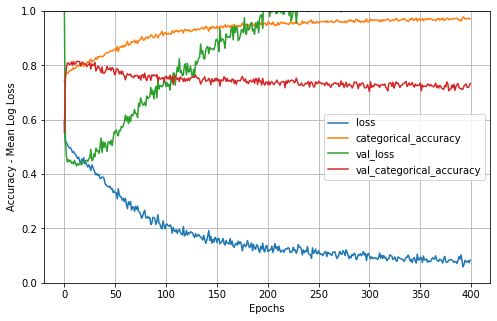
\includegraphics[scale=0.5]{n-tr-ax-ey.png}		
					\caption{Entrenamiento durante el Experimento y de la Arquitectura x}	
					\label{n-tr-a4-e3}
				\end{center}
			\end{figure}
			
			Bla bla bla
			%Imagen de la matriz de confusion, labels IMPORTANTES
			%Nombre de la imagen de la matriz n-cm-ax-ey.png
			\begin{figure}[!h]
				\begin{center}
					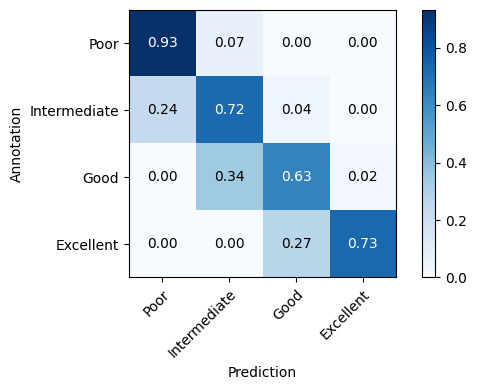
\includegraphics[scale=0.7]{n-cm-ax-ey.png}		
					\caption{Matriz de confusi\'on en el Experimento y de la Arquitectura x}	
					\label{n-cm-a4-e3}
				\end{center}
			\end{figure}
\end{document}
